\documentclass{beamer}
\mode<presentation>
\usepackage{amsmath}
\usepackage{amssymb}
%\usepackage{advdate}
\usepackage{adjustbox}
\usepackage{subcaption}
\usepackage{enumitem}
\usepackage{multicol}
\usepackage{mathtools}
\usepackage{listings}
\usepackage{url}
% \usepackage{minted}
% \usepackage{gvv}

\usepackage{tcolorbox}
\tcbuselibrary{minted,breakable,xparse,skins}



\definecolor{bg}{gray}{0.95}
\DeclareTCBListing{mintedbox}{O{}m!O{}}{%
  breakable=true,
  listing engine=minted,
  listing only,
  minted language=#2,
  minted style=default,
  minted options={%
    linenos,
    gobble=0,
    breaklines=true,
    breakafter=,,
    fontsize=\scriptsize,
    numbersep=8pt,
    #1},
  boxsep=0pt,
  left skip=0pt,
  right skip=0pt,
  left=25pt,
  right=0pt,
  top=3pt,
  bottom=3pt,
  arc=5pt,
  leftrule=0pt,
  rightrule=0pt,
  bottomrule=2pt,
  toprule=2pt,
  colback=bg,
  colframe=orange!70,
  enhanced,
  overlay={%
    \begin{tcbclipinterior}
    \fill[orange!20!white] (frame.south west) rectangle ([xshift=20pt]frame.north west);
    \end{tcbclipinterior}},
  #3,
}


\def\UrlBreaks{\do\/\do-}
\usetheme{Madrid}
\usecolortheme{lily}
\setbeamertemplate{footline}
{
  \leavevmode%
  \hbox{%
  \begin{beamercolorbox}[wd=\paperwidth,ht=2.25ex,dp=1ex,right]{author in head/foot}%
    \insertframenumber{} / \inserttotalframenumber\hspace*{2ex} 
  \end{beamercolorbox}}%
  \vskip0pt%
}
\setbeamertemplate{navigation symbols}{}

\providecommand{\nCr}[2]{\,^{#1}C_{#2}} % nCr 
\providecommand{\nPr}[2]{\,^{#1}P_{#2}} % nPr
\providecommand{\mbf}{\mathbf}
\providecommand{\pr}[1]{\ensuremath{\Pr\left(#1\right)}}
\providecommand{\qfunc}[1]{\ensuremath{Q\left(#1\right)}}
\providecommand{\sbrak}[1]{\ensuremath{{}\left[#1\right]}}
\providecommand{\lsbrak}[1]{\ensuremath{{}\left[#1\right.}}
\providecommand{\rsbrak}[1]{\ensuremath{{}\left.#1\right]}}
\providecommand{\brak}[1]{\ensuremath{\left(#1\right)}}
\providecommand{\lbrak}[1]{\ensuremath{\left(#1\right.}}
\providecommand{\rbrak}[1]{\ensuremath{\left.#1\right)}}
\providecommand{\cbrak}[1]{\ensuremath{\left\{#1\right\}}}
\providecommand{\lcbrak}[1]{\ensuremath{\left\{#1\right.}}
\providecommand{\rcbrak}[1]{\ensuremath{\left.#1\right\}}}
\theoremstyle{remark}
\newtheorem{rem}{Remark}
\newcommand{\sgn}{\mathop{\mathrm{sgn}}}
\providecommand{\abs}[1]{\left\vert#1\right\vert}
\providecommand{\res}[1]{\Res\displaylimits_{#1}} 
\providecommand{\norm}[1]{\lVert#1\rVert}
\providecommand{\mtx}[1]{\mathbf{#1}}
\providecommand{\mean}[1]{E\left[ #1 \right]}
\providecommand{\fourier}{\overset{\mathcal{F}}{ \rightleftharpoons}}
%\providecommand{\hilbert}{\overset{\mathcal{H}}{ \rightleftharpoons}}
\providecommand{\system}{\overset{\mathcal{H}}{ \longleftrightarrow}}
	%\newcommand{\solution}[2]{\textbf{Solution:}{#1}}
%\newcommand{\solution}{\noindent \textbf{Solution: }}
\providecommand{\dec}[2]{\ensuremath{\overset{#1}{\underset{#2}{\gtrless}}}}
\newcommand{\myvec}[1]{\ensuremath{\begin{pmatrix}#1\end{pmatrix}}}
\let\vec\mathbf

\lstset{
%language=C,
frame=single, 
breaklines=true,
columns=fullflexible
}

\numberwithin{equation}{section}

\title{Matgeo Presentation}
\author{Pushkar Gudla \\ AI24BTECH11012\\IIT Hyderabad.}
\date{\today} 

\begin{document}

\begin{frame}
\titlepage
\end{frame}

\section*{Outline}
\begin{frame}{Contents}
\tableofcontents    
\end{frame}

\section{Problem}
\begin{frame}{Problem Statement}
    The area of the region bounded by the curve $x^2=4y$ and the straight line $x=4y-2$ is
\end{frame}

\section{Solution}
\subsection{Setup and Variable Definitions}
\begin{frame}{Setup and Variable Definitions}
\begin{table}[h!]    
  \centering
  \begin{tabular}[15pt]{ |c| c|}
    \hline
    \textbf{Variable} & \textbf{Description}\\ 
    \hline
    $a$ & Length of side $BC$ \\
    \hline 
    $b$ & Length of side $AC$ \\
	\hline
    $c$ & Length of side $AB$ \\
    \hline
	$k$ & $k=b-c$ \\
	\hline
    \end{tabular}

  \caption{Variables and given data}
\end{table}
\end{frame}

\subsection{Converting to Matrix form}
\begin{frame}{Converting the equations to Matrix form}
    To simplify the calculation of points of intersection, the curve $x^2=4y$ is represented in standard conic matrix form:
    \begin{align}
        g(x) &= x^\top \vec{V}x + 2\vec{u}^\top x + f=0\\
        \vec{V} &= \myvec{1 & 0\\0 & 0}\\
	\vec{u} &= \myvec{0\\2}\\
	f &= 0
    \end{align}
\end{frame}

\subsection{Parametric Form of the Line}
\begin{frame}{Parametric Form of the Line}
	\begin{align}
	L: \vec{x} &= \vec{h}+k\vec{m} 
 \end{align}
 where $k$ is a scalar constant\\
 \begin{align}
        \vec{h} &= \myvec{-2 \\ 0}\\
	\vec{m} &= \myvec{1 \\ \frac{1}{4}}\\
	\vec{x_i} &= \vec{h}+k_{i}\vec{m}
 \end{align}
\end{frame}

\subsection{Finding Points of Intersection}
\begin{frame}{Finding Points of Intersection}
On substituting $L$ in $g(x)$ we get a quadratic equation in $k$. We find that the discriminant is not equal to zero and thus we get two values $k_1$ and $k_2$.
The point obtained by substituting $k_1$ in $L$ is $\vec{x_1}$ and similarly on substituting $k_2$ in $L$ we get $\vec{x_2}$.
\begin{align}
	k_1 &= \frac{1}{\vec{m}^\top \vec{V}\vec{m}}\brak{-m^\top\brak{\vec{V}\vec{h}+\vec{u}}+ \sqrt{[\vec{m}^\top \brak{\vec{V}\vec{h}+\vec{u}}]^2 - g(\vec{h})\brak{\vec{m}^\top\vec{V}\vec{m}}}} \\
	k_2 &= \frac{1}{\vec{m}^\top \vec{V}\vec{m}}\brak{-m^\top\brak{\vec{V}\vec{h}+\vec{u}}- \sqrt{[\vec{m}^\top \brak{\vec{V}\vec{h}+\vec{u}}]^2 - g(\vec{h})\brak{\vec{m}^\top\vec{V}\vec{m}}}}
\end{align}
On solving for $k_1$ and $k_2$ we get $k_1=4$ and $k_2=1$. Thus
\begin{align}
    \vec{x_1} &= \myvec{2\\1}\\
    \vec{x_2} &= \myvec{-1\\ \frac{1}{4}}
\end{align}
\end{frame}

\subsection{Finding Area through Integration}
\begin{frame}{Finding Area through Integration}
    The area between the curve and the line from $x=-1$ to $x=2$ is calculated using the following integration:\\
    Area = $\int_{-1}^{2}\brak{\frac{x}{4}+\frac{1}{2}-\frac{x^2}{4}}dx$\\
    Solving this integral, we get Area=$\frac{9}{8}$.\\
    Hence, the area bound between the curve $x^2=4y$ and the line $x=4y-2$ is $\frac{9}{8}$.
\end{frame}

\section{Codes}
\subsection{C code to verify the Area}

\begin{frame}[fragile,allowframebreaks]
\frametitle{C code to verify the Area}
\begin{mintedbox}{c}[break at=.8\textheight]
#include <stdio.h>
#include <math.h>

// Define the functions for the curve and the line
double curve(double x) {
    return x * x / 4.0;  // y = x^2 / 4
}

double line(double x) {
    return (x + 2) / 4.0;  // y = (x + 2) / 4
}

// Numerical integration using the trapezoidal rule
double integrate(double (*f1)(double), double (*f2)(double), double a, double b, int n) {
    double h = (b - a) / n;  // Step size
    double area = 0.0;

    for (int i = 0; i < n; i++) {
        double x1 = a + i * h;
        double x2 = a + (i + 1) * h;

        // Area of trapezoid between the functions
        double y1 = f2(x1) - f1(x1);
        double y2 = f2(x2) - f1(x2);

        area += 0.5 * (y1 + y2) * h;
    }

    return area;
}

int main() {
    // Define integration bounds
    double a = -1.0;
    double b = 2.0;
    int n = 10000;  // Number of intervals for better accuracy

    // Calculate area
    double area = integrate(curve, line, a, b, n);

    // Write result to area.txt
    FILE *file = fopen("area.txt", "w");
    if (file != NULL) {
        fprintf(file, "Area between the curve and the line: %f\n", area);
        fclose(file);
        printf("Area has been written to area.txt\n");
    } else {
        printf("Error opening file!\n");
    }

    return 0;
}

  \end{mintedbox}
\end{frame}

\subsection{Generating Parabola using C}
\begin{frame}[fragile,allowframebreaks]
\frametitle{Generating Parabola using C}
  \begin{mintedbox}{c}[break at=.8\textheight]
#include <stdio.h>
#include <math.h>

int main() {
    FILE *file;
    file = fopen("parabola_points.txt", "w");

    if (file == NULL) {
        printf("Error opening file!\n");
        return 1;
    }

    // Generate points for the parabola x^2 = 4y
    float x, y;
    float step = 0.1;  // Step size for x
    float x_max = 5;  // Maximum value of x (you can adjust as needed)

    for (x = -x_max; x <= x_max; x += step) {
        y = (x * x) / 4.0;
        fprintf(file, "%f %f\n", x, y);
    }

    fclose(file);
    printf("Points have been written to parabola_points.txt\n");
    return 0;
}
}
  \end{mintedbox}
  
  \end{frame}
  
  \subsection{Plotting the figure using Python}
\begin{frame}[fragile,allowframebreaks]
\frametitle{Plotting the figure using Python}
   \begin{mintedbox}{Python}[break at=.8\textheight]
import sys                                  
sys.path.insert(0, '/home/pushkar/matgeo/codes/CoordGeo')    
import numpy as np
import numpy.linalg as LA
import matplotlib.pyplot as plt
import matplotlib.image as mpimg

from line.funcs import *
from conics.funcs import *
from triangle.funcs import *
import params
A = np.array([2,1])
B = np.array([-1, 0.25])
import matplotlib.pyplot as plt

# Initialize lists for x and y coordinates
x_vals = []
y_vals = []

# Read points from the file
with open("parabola_points.txt", "r") as file:
    for line in file:
        x, y = map(float, line.split())
        x_vals.append(x)
        y_vals.append(y)

# Plot the points
plt.plot(x_vals, y_vals, label="$x^2 = 4y$")
plt.xlabel('x')
plt.ylabel('y')
plt.title('Parabola: $x^2 = 4y$')

# use set_position
ax = plt.gca()
ax.spines['top'].set_color('none')
ax.spines['left'].set_position('zero')
ax.spines['right'].set_color('none')
ax.spines['bottom'].set_position('zero')

#Plotting all line

# Define the range of y values
y = np.linspace(-1, 2, 100)

# Define the equation x = 4y - 2
x = 4 * y - 2

# Create the plot
plt.plot(x, y, label='x = 4y - 2')



#Labeling the coordinates
tri_coords = np.vstack((A,B)).T
plt.scatter(tri_coords[0,:], tri_coords[1,:])
vert_labels = ['A(2,1)','B(-1,0.25)']
for i, txt in enumerate(vert_labels):
       plt.annotate(txt,      # this is the text
                 (tri_coords[0,i], tri_coords[1,i]), # this is the point to label
                 textcoords="offset points",   # how to position the text
                 xytext=(0,10),     # distance from text to points (x,y)
                 ha='center')     # horizontal alignment can be left, right or center


#plt.fill_between(x1,x2,O,color='green', alpha=.2)
plt.xlabel('$x$')
plt.ylabel('$y$')
plt.legend(loc='best')
plt.grid(True) # minor
plt.axis('equal')
plt.savefig('plot')

  \end{mintedbox}
\end{frame}

\section{Figure}
\begin{frame}{Figure}
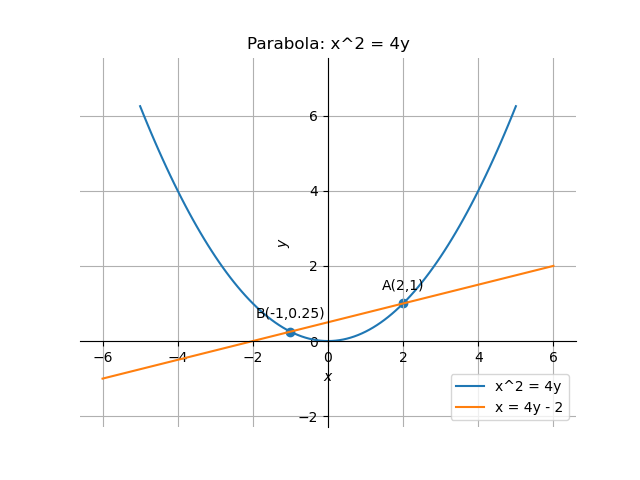
\includegraphics[width=0.8\textwidth]{figs/plot.png}
\end{frame}

\end{document}

